\section{Parametric Solution}
\label{sec:parametric}

In modeling electromechanical transport, it is important to distinguish between
\emph{geometric effects} and \emph{material effects}. Geometric changes arise from
deformation of the domain (e.g., changes in length $L$ or cross-sectional area $A$),
which influence quantities such as resistance through the relation
\begin{equation}
    R = \frac{L}{A\,\sigma}.
    \label{eq:resistance}
\end{equation}
Material effects, in contrast, describe how intrinsic properties, such as the
electrical conductivity $\sigma$, change due to deformation. In semiconductors,
this latter effect---known as \emph{piezoresistivity}---is typically dominant
and is the focus of the present work.

To incorporate this dependence, the conductivity is treated as a function of the
mechanical strain,
\begin{equation}
    \sigma = \sigma(\varepsilon),
    \label{eq:sigma_eps}
\end{equation}
where $\varepsilon$ denotes a scalar strain measure derived from the strain tensor
$\varepsilon(\mathbf{u})$ introduced in Section~\ref{sec:math model}.\footnote{In the
one-dimensional setting considered here, $\varepsilon$ reduces to the axial
component $\varepsilon_{xx}$; the generalization to tensorial strain is
straightforward through the appropriate invariants.} The exact functional form of
$\sigma(\varepsilon)$ is generally unknown or analytically intractable when
derived from first-principles microscopic transport theory. For sufficiently
small deformations, however, $\sigma(\varepsilon)$ may be assumed smooth and
approximated by its Taylor expansion about the undeformed reference state
$\varepsilon = 0$:
\begin{equation}
    \sigma(\varepsilon)
    \approx \sigma_0
    + \left.\frac{d\sigma}{d\varepsilon}\right|_{0}\!\varepsilon
    + \frac{1}{2}\left.\frac{d^2\sigma}{d\varepsilon^2}\right|_{0}\!\varepsilon^{2}
    + \mathcal{O}(\varepsilon^{3}),
    \label{eq:taylor_raw}
\end{equation}
where $\sigma_0 = \sigma(0)$ is the reference (unstrained) conductivity.

Factoring out $\sigma_0$ yields the normalized form
\begin{equation}
    \sigma(\varepsilon)
    = \sigma_0\left(1 + \pi\,\varepsilon + \alpha\,\varepsilon^{2} + \dots\right),
    \label{eq:taylor_normalized}
\end{equation}
with the dimensionless coefficients
\begin{equation}
    \pi = \frac{1}{\sigma_0}\left.\frac{d\sigma}{d\varepsilon}\right|_{0},
    \qquad
    \alpha = \frac{1}{2\,\sigma_0}\left.\frac{d^2\sigma}{d\varepsilon^{2}}\right|_{0}.
    \label{eq:coeff_def}
\end{equation}
Here $\pi$ is the \emph{linear piezoresistive coefficient}, characterizing the
first-order sensitivity of the conductivity to strain, while $\alpha$ captures
higher-order nonlinear effects relevant at larger strain amplitudes. The
expansion~\eqref{eq:taylor_normalized} is not geometric in nature; rather, it
provides a local approximation of how the \emph{internal electronic transport
properties} of the material respond to deformation.

\begin{figure}[ht]
    \centering
    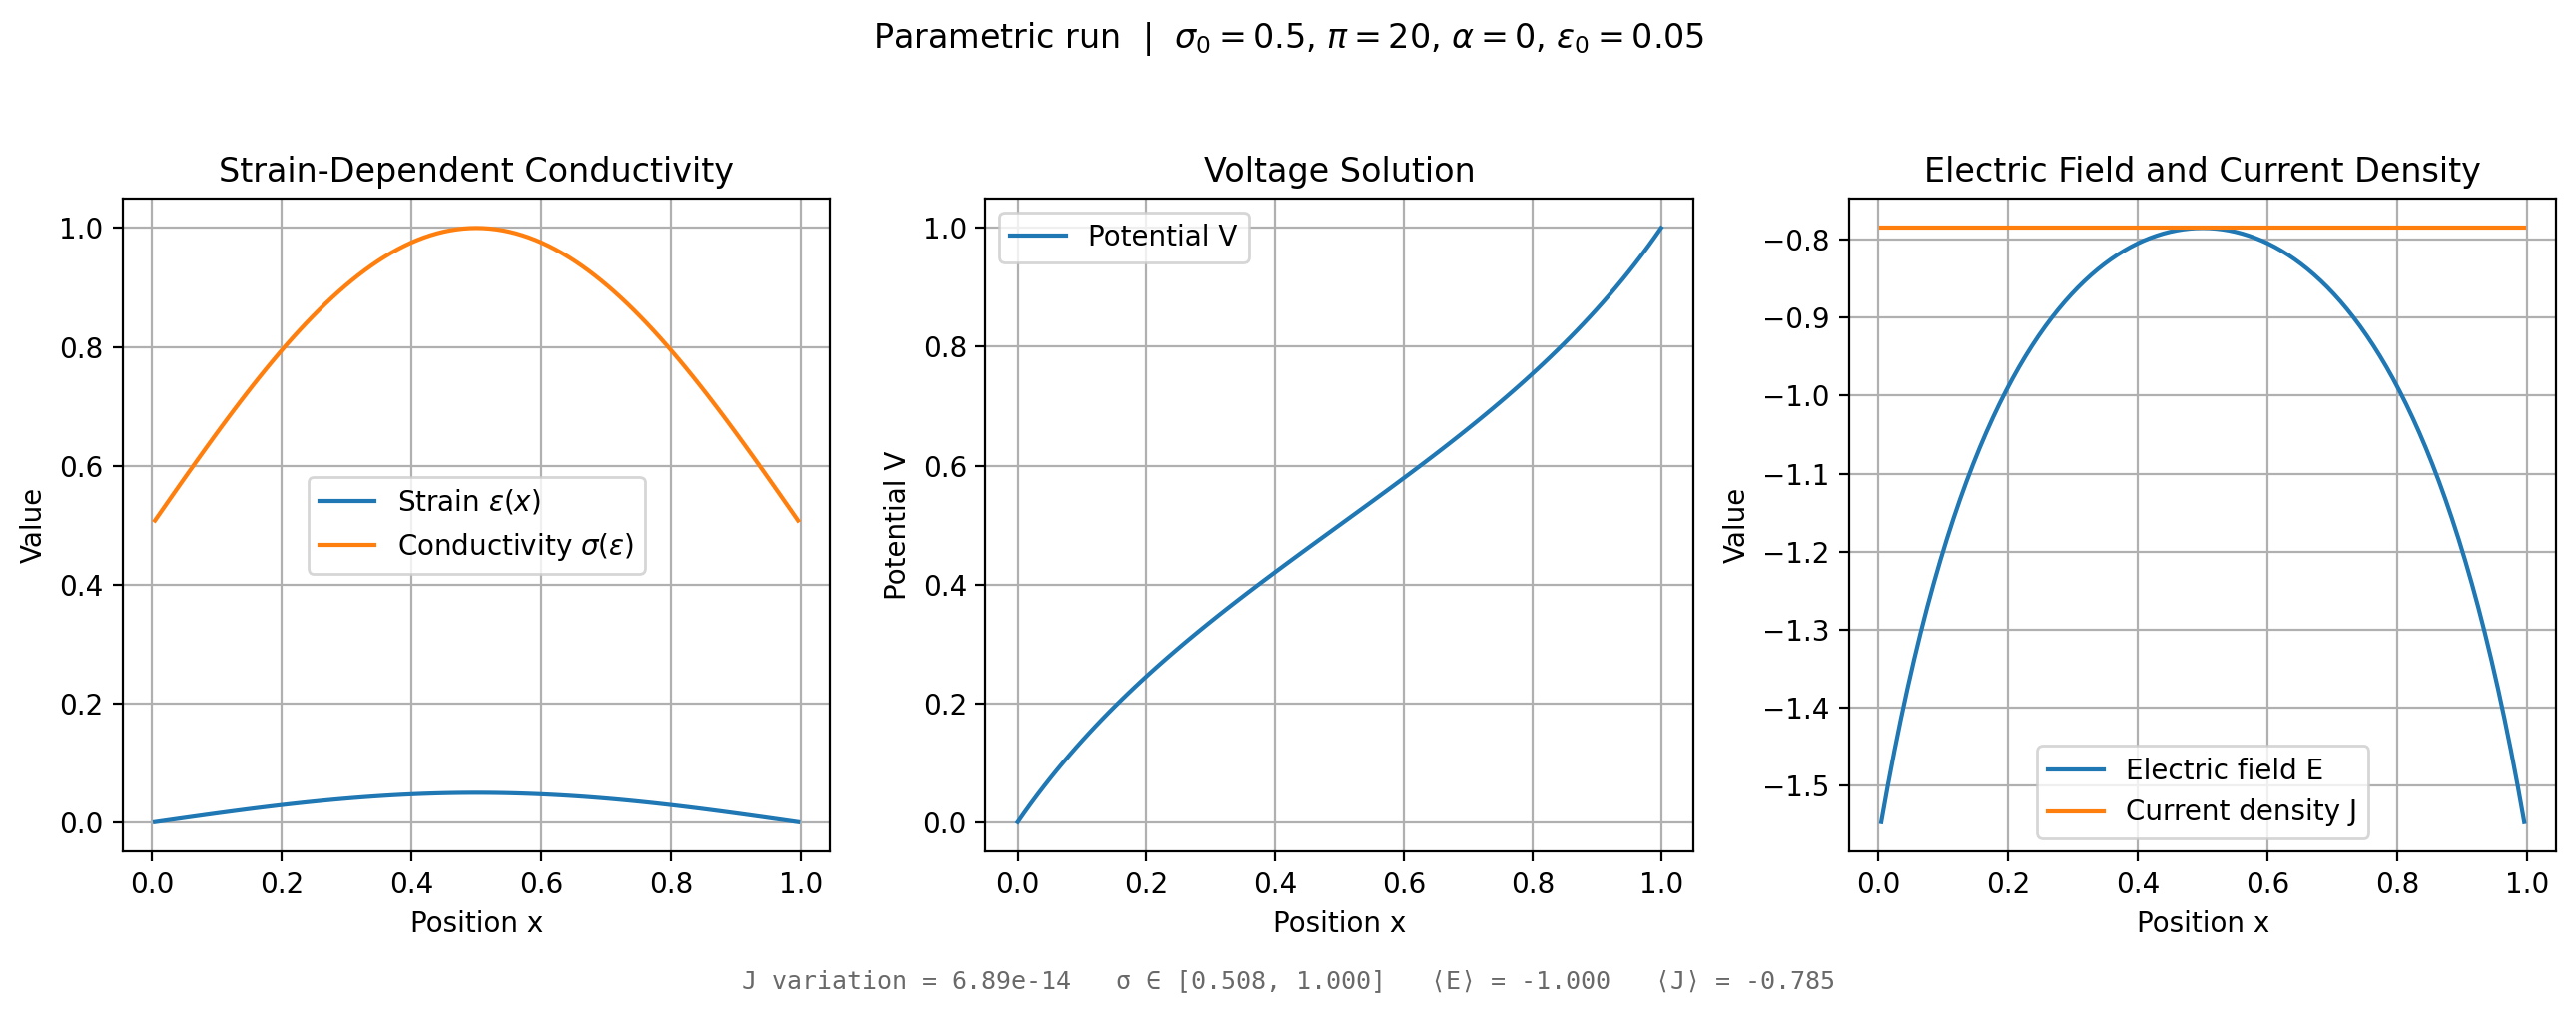
\includegraphics[width=0.75\textwidth]{Images/par_s0=0.5_pi=p20_a=p0_e0=0.05.png}
    %\fbox{\parbox[c][4cm][c]{0.75\linewidth}{\centering\textit{Placeholder: 
    %$\sigma(\varepsilon)$ vs.\ $\varepsilon$ for varying $\pi$ and $\alpha$.}}}
    \caption{Normalized conductivity $\sigma(\varepsilon)/\sigma_0$ as a function
    of strain $\varepsilon$ for representative values of the linear coefficient
    $\pi$ and the nonlinear coefficient $\alpha$. For small $|\varepsilon|$ the
    response is dominated by the linear term; the quadratic contribution becomes
    visible at larger strain amplitudes.}
    \label{fig:sigma_vs_eps}
\end{figure}



Physically, mechanical strain modifies the crystal lattice, which in turn alters
the electronic band structure, the carrier effective masses, and the dominant
scattering mechanisms. Within the Drude picture, the conductivity reads
\begin{equation}
    \sigma = \frac{n\,e^{2}\,\tau}{m^{*}},
    \label{eq:drude}
\end{equation}
where $n$ is the carrier density, $e$ the elementary charge, $\tau$ the momentum
relaxation time, and $m^{*}$ the effective mass. Strain therefore enters
$\sigma$ through all three microscopic quantities $n$, $\tau$, and $m^{*}$
simultaneously. Consequently, the Taylor expansion~\eqref{eq:taylor_normalized}
should be understood as an effective continuum-level description that subsumes
these microscopic contributions into the macroscopic coefficients $\pi$ and
$\alpha$, without requiring an explicit microscopic derivation.

\begin{figure}[ht]
    \centering
    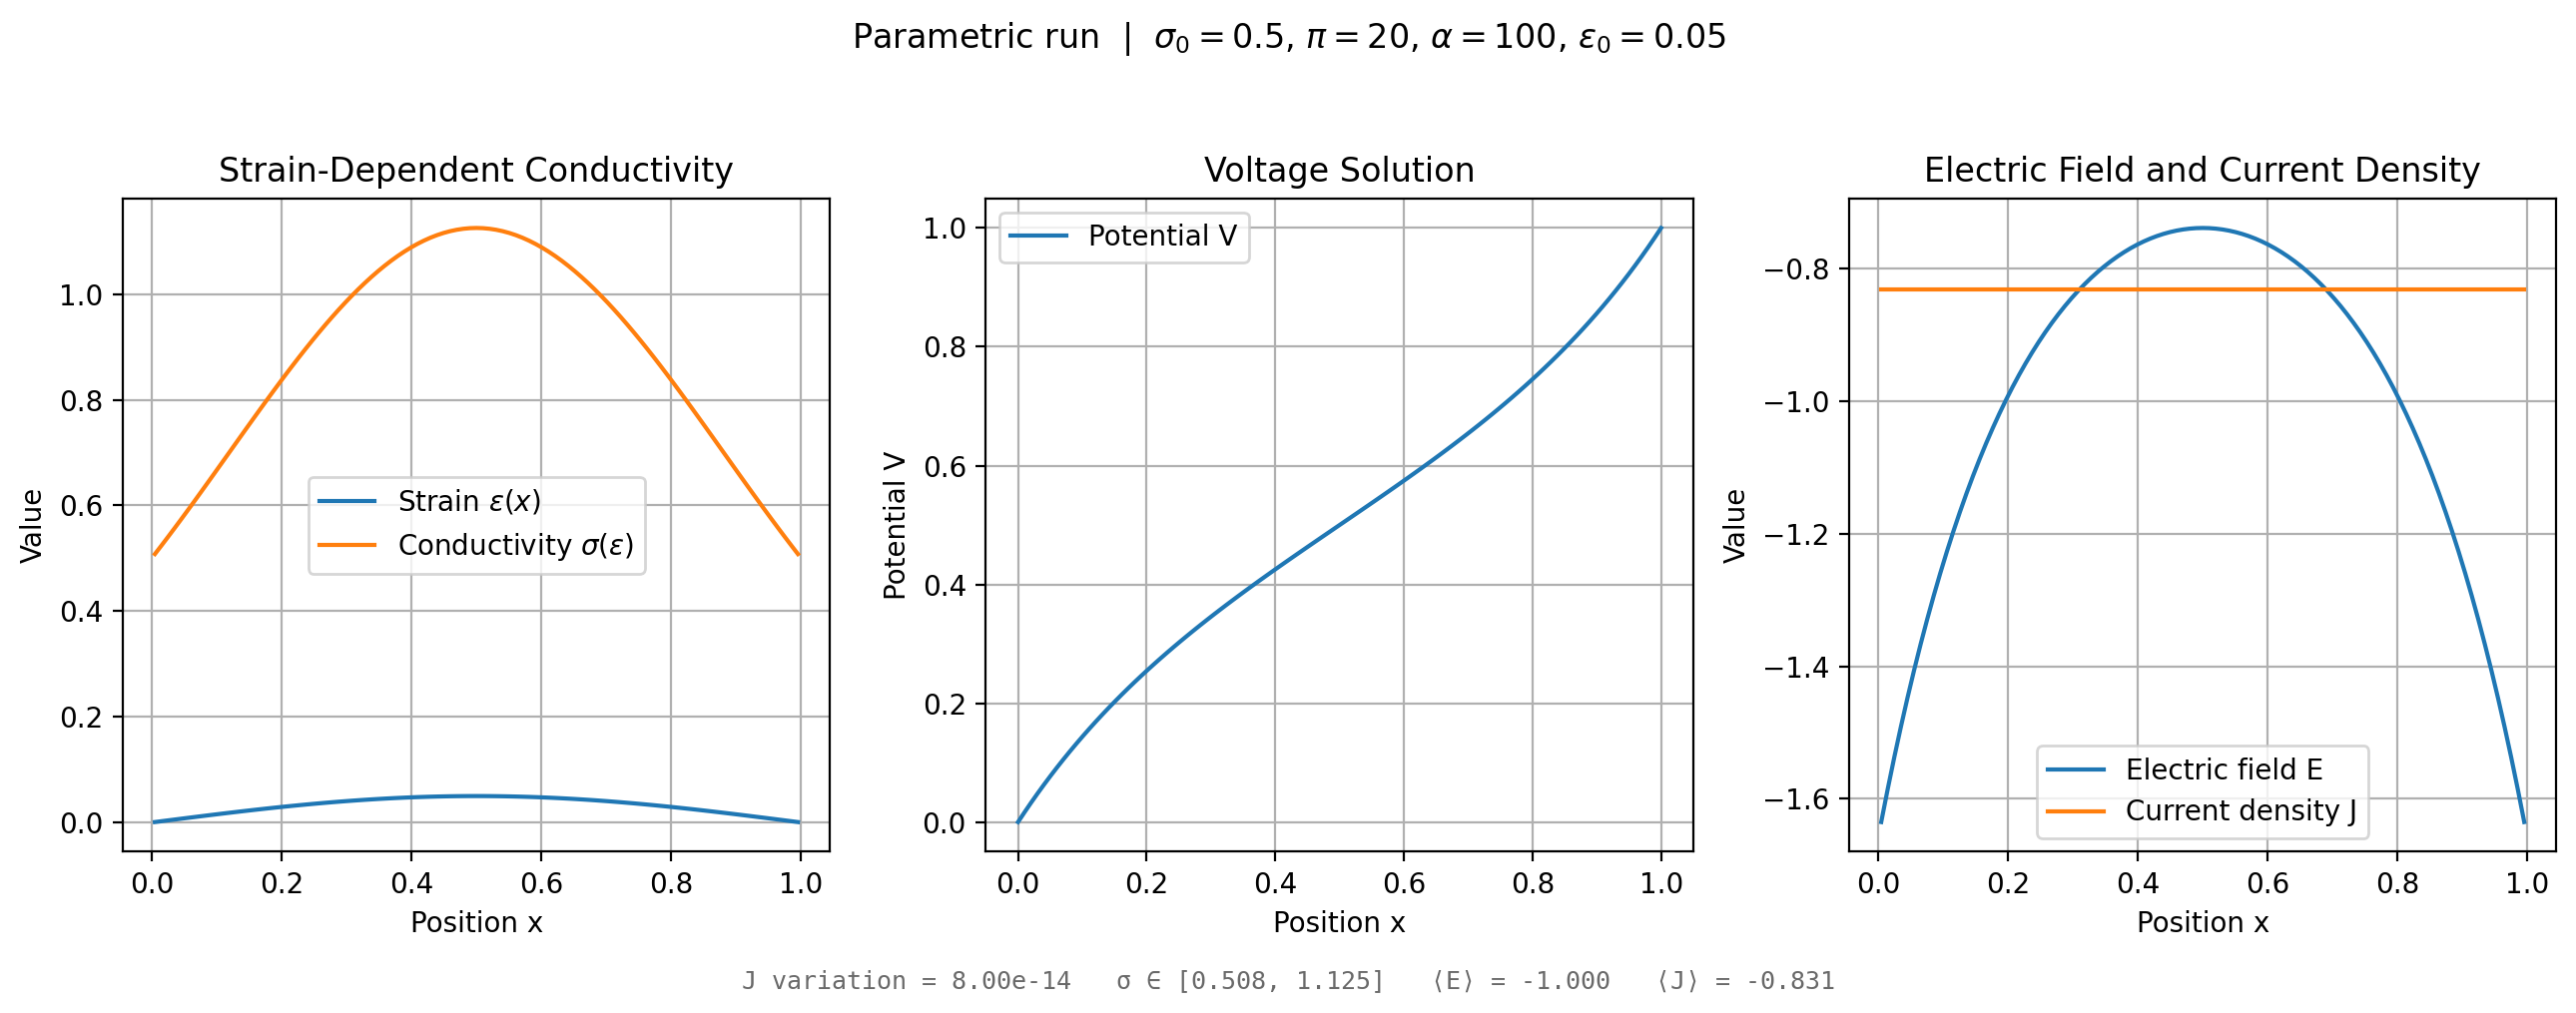
\includegraphics[width=0.75\textwidth]{Images/par_s0=0.5_pi=p20_a=p100_e0=0.05.png}
    %\fbox{\parbox[c][5cm][c]{0.85\linewidth}{\centering\textit{Placeholder:
    %Potential $V(x)$, electric field $E(x)$, and current density $J(x)$ for the
    %parametric study.}}}
    \caption{Finite element results for the one-dimensional coupled problem with
    strain-dependent conductivity~\eqref{eq:taylor_normalized}. A prescribed
    strain field $\varepsilon(x) = \varepsilon_0 \sin(\pi x)$ is used to
    illustrate the effect of the coefficients $\pi$ and $\alpha$ on the
    potential, electric field, and current density. The current density remains
    constant up to machine precision, confirming current conservation.}
    \label{fig:parametric_study}
\end{figure}

The parametric study based on~\eqref{eq:taylor_normalized} reveals a clear
separation between uncoupled and coupled regimes. For $\pi = \alpha = 0$ the
conductivity reduces to the constant baseline $\sigma = \sigma_0$, recovering a
linear potential profile $V(x)$, a constant electric field, and a uniform
current density; strain is present but does not influence transport. A non-zero
linear coefficient $\pi$ activates first-order piezoresistive coupling: the
conductivity now responds directly to the strain field, the electric field
redistributes accordingly, and the potential profile becomes nonlinear, while
the current density remains spatially constant in accordance with charge
conservation,
\begin{equation}
    \frac{dJ}{dx} = 0.
    \label{eq:current_cons}
\end{equation}
The sign and magnitude of $\pi$ control whether the conductivity locally
increases or decreases under deformation, and thereby the sensitivity of the
electrical response. The quadratic term $\alpha\varepsilon^{2}$ introduces
additional curvature in $\sigma(\varepsilon)$ and is typically subdominant for
small strains, but becomes appreciable at larger amplitudes. In all cases the
admissibility condition $\sigma(\varepsilon) > 0$ must be respected to preserve
physical meaning.

Across the tested configurations, the numerical results confirm that the current
density is conserved to machine precision, validating the finite element
implementation. The simulations show that the system maintains equilibrium by
compensating local variations in conductivity with corresponding adjustments in
the electric field, consistent with the constitutive relation $J = \sigma E$.
Representative parameter ranges for stable exploration are
$\sigma_0 \in [0.1, 2.0]$, $\pi \in [5, 20]$, $\alpha \in [0, 100]$, and strain
amplitudes $\varepsilon_0 \in [10^{-3}, 10^{-2}]$. Within this regime, the model
captures both linear and nonlinear piezoresistive behavior while remaining
numerically robust and physically interpretable.